\documentclass[a4paper,12pt]{article}
\usepackage[margin=0.75in]{geometry}
\usepackage[hungarian]{babel}
\usepackage{tikz}
\usepackage{minted}
\usepackage{graphicx}
\usepackage{wrapfig}
\usepackage{float}
\usepackage{tabularx}
\usepackage{colortbl}
\usepackage{tabularray}
\usepackage{animate}
\graphicspath{{./images/}}

\newcolumntype{Y}{>{\centering\arraybackslash}X}

\title{\huge{Programozási technológia} \\ \large  III. Beadandó feladat}
\author{Boda Bálint \\ KDHPNI}
\date{2022. 12. 11}

\begin{document}
	\maketitle
	\section{Feladat}
	Készítsünk programot, amellyel a Tronból ismert fény-motor párbajt játszhatjuk felülnézetből. Két játékos játszik egymás ellen egy-egy olyan motorral, amely fénycsíkot húz maga mögött a képernyőn. A motor minden másodpercben a legutoljára beállított irányba halad feltéve, hogy a játékos nem változtatja meg azt egy megfelelő billentyű lenyomásával. (WASD az első játékos, nyilak a második játékos.)
	\\[8pt] \noindent
	Az a játékos veszít, aki előbb neki ütközik a másik játékos fénycsíkjának vagy a képernyő szélének. A játék elején kérjük el a játékosok nevét és engedjük meg, hogy maguk válasszák ki a fényük színét. A játék végekor a győztes játékos eredményét növeljük meg az adatbázisban. Ha a játékos még nem található meg az adatbázisban, úgy szúrjunk be egy új sort. Egy menüpontban legyen lehetőségünk a 10 legjobb eredménnyel rendelkező játékost megtekinteni, az elért pontszámukkal, továbbá lehessen bármikor új játékot indítani egy másik menüből.
	\newpage
	\section{Terv}
	\subsection{A feladat elemzése}
	A játék létrehozásához a következőket kell megvalósítani:
	\begin{itemize}
		\item időzítő
		\begin{itemize}
			\item vizuális megjelenítés, másodpercenként a játék előrevitele
		\end{itemize}
		\item játékosok
		\begin{itemize}
			\item játékosnév megadása (ellenőrzés, hogy ne legyen a két játékos neve ugyan az)
			\item mozgás, fénycsík létrehozása
			\item fénycsík színének megadása (ellenőrzés, hogy ne legyen a két fénycsík ugyan olyan színű, ne olvadjon be a környezetbe)
			\item ütközés érzékelése
		\end{itemize}
		\item játéktér
		\begin{itemize}
			\item generálás
		\end{itemize}
		\item adatbázis
		\begin{itemize}
			\item eredménye eltárolása adatbázisba
			\item eredmények lekérése adatbázisból
		\end{itemize}
		\item grafikus kezelőfelület
		\begin{itemize}
			\item játékos adatok bevitele
			\item új játék kezdése
			\item adatbázisból lekért adatok megjelenítése
		\end{itemize}
	\end{itemize}
	\subsection{Típusok}
	\subsubsection{Direction}
	Az irány enumeráció konstansaival a játékosok haladásának irányát reprezentáljuk. Lehetséges értékei: \mintinline{java}|UP|, \mintinline{java}|LEFT|, \mintinline{java}|DOWN|, \mintinline{java}|RIGHT|.
	\subsubsection{Player}
	A játékosokat nevükkel, színükkel, vízszintes és függőleges pozíciójukkal és mozgásuk irányával reprezentáljuk. A játékosok tulajdonságai lekérhetőek, képesek irányt váltani és a jelenlegi irányba haladni.
	\subsubsection{Tile}
	A \mintinline{java}|Tile| osztály a játéktér egy celláját reprezentálja, egyetlen adattagot tartalmaz, ami a mező színe. Ezen szín alapján dönthető, el, hogy a cella biztonságos-e. A biztonságos cellákat színe az $ (41, 53, 66) $ RGB kódú szín, melyet egy osztályszintű konstansban tárolunk el \mintinline{java}|SAFE_COLOR| néven. Az összes többi cellát nem biztonságosnak tekintünk.
	\subsubsection{GameModel}
	A játék modellje, eltárolja a játékosokat, a játékteret, és egy az adatbázissal kommunikáló objektumot.
	\\[4pt]
	A modell a játékteret a következő algoritmus alapján állítja elő:
	\begin{enumerate}
		\item{
			A térkép bal felső negyedében (beleértve a két negyed közti cellákat is) kiválaszt egy koordinátát. Például $7 \times 7$-es pályaméret esetén:
			\begin{figure}[H]
				\centering
				\begin{tblr}{
						rows = {1.25em, rowsep = 2pt},
						columns = {1.25em, colsep = 2pt},
						cells = {m,c},
						cell{1,9}{1-9} = {black},
						cell{2-8}{1,9} = {black},
						cell{2-5}{2-5} = {teal},
						hlines,
						vlines,
					}
					& & & & & & & & \\ 
					& & & & & & & & \\ 
					& & & & & & & & \\ 
					& & & & & & & & \\ 
					& & & & & & & & \\
					& & & & & & & & \\ 
					& & & & & & & & \\
					& & & & & & & & \\
					& & & & & & & & \\ 
				\end{tblr}	
			\end{figure}
			a zöld cellatartomány egy koordinátáját választja ki.
		}
		\item{
			előállít egy gyűjteményt, melyben a kiválasztott koordináta körüli koordináták és a maga a koordináta kerül
		}
		\item{
			összekeveri a gyűjteményt
		}
		\item{
			generál egy $n \in [3..9]$ számot, majd veszi a gyűjtemény első $n$ elemét (a többi koordinátát eldobja) 
		}
		\item{
			végigiterál a koordináta gyűjteményen és feketére színezi (ezáltal nem biztonságossá teszi) a játéktér adott $(x,y)$ koordinátájú mezőjét és annak középpontos tükörképét. Legyen $v$ a pálya vízszintes $f$ a pálya függőleges mérete, ekkor az $(x,y)$ pont tükörképe az
			\[ \Bigl( (v - 1 - x), (f - 1 - y) \Bigr) \]
			pont.
		}
		\item{
			megismétli a 2-5. lépéseket egy jobb felső negyedbeli (beleértve a negyedek közti cellákat is) koordinátával.
		}
		\item{
			a játékosok körüli $ 3 \times 3 $-as területet biztonságossá teszi, azon cellák kivételével, melyek a játéktér szélei
		}
	\end{enumerate}
	Ezen osztály \mintinline{java}|doRound()| metódusa felel a játék egy körének szimulálásáért, ami egy \mintinline{java}|GameState|-et ad vissza.
	\subsubsection{GameState}
	A Játék állapotát reprezentáló enumeráció. Lehetséges értékei: \mintinline{java}|IN_PROGRESS|, \mintinline{java}|PLAYER1WON|, \mintinline{java}|PLAYER2WON|, \mintinline{java}|DRAW|.
	\subsubsection{HighScore}
	Egy rekord mely, egy nevet (\mintinline{java}|String|) és egy pontszámot (\mintinline{java}|int|) tárol el.
	\subsubsection{HighScores}
	Az játék adatbázisával kommunikáló osztály. Az adatbázis formátuma:
	\begin{figure}[H]
		\centering
		\begin{tabular}{|c|c|}
			\hline
			oszlopnév & adattípus  \\
			\hline
			id & INT  \\
			\hline
			name & TINYTEXT \\
			\hline
			score & INT\\
			\hline
		\end{tabular}
	\end{figure} \noindent
	Ahol \mintinline{sql}|id| automatikusan növekedő elsődleges kulcs. Az osztály lehetővé teszi új eredmények beszúrását és a legjobb eredmények lekérdezését. Az osztály egyke tervmintát használ.
	\subsubsection{GameView}
	A \mintinline{java}|JFrame| osztályból származtatott osztály, mely a játék ablakát valósítja meg. Ezen osztály végzi az alkalmazás többi menüpontjának példányosítását, és az ezek közti váltás megvalósítását. 
	\subsubsection{MainMenu}
	A \mintinline{java}|MainMenu| osztály egy \mintinline{java}|JPanel|, ami a játék főmenüjét alkotja. A főmenüből lehetőségünk van testreszabni a játékosokat, új játékot kezdeni, megadni a pályaméretet, megtekinteni az eredményeket és kilépni a játékból.
	\\[4pt]
	A főmenü eseménykezelői:
	\begin{figure}[H]	
		\centering
		\begin{tblr}{colspec={|X|X[3]|}, row{1} = {c}, hlines, cells={m,c},}
			Esemény            & Tevékenység \\
			Játék indítás gomb & A főmenüben megadott adatok alapján új játék próbál indulni, ha sikertelen hibaüzenet jelenik meg, ha sikeres a nézet átvált a játékra. Újraindul az időzítő. \\
			Eredmények gomb    & A nézet átvált az eredmények fülre. \\
			Kilépés gomb       & A program kilép. \\
		\end{tblr}
	\end{figure}
	
	\subsubsection{PlayerCustomizationPanel}
	Ezen osztály példányai a játékosok testreszabás menüjeit valósítják meg. Lehetőség van megadni a játékos nevét és fénycsíkjának színét. A menüben továbbá megjelenik, hogy az adott játékos, mely billentyűkkel irányítható.
	\newpage
	\subsubsection{GameMenu}
	A konkrét játék menüje. Amikor az alkalmazás nézetet erre a panelre vált, elindul a egy időzítő, mely minden másodpercben előidéz egy eseményt ami lépteti a játék állapotát. A játék eseménykezelői.
	\begin{figure}[H]	
		\centering
		\begin{tblr}{colspec={|X|X[3]|}, row{1} = {c}, hlines, cells={m,c},}
			Esemény            & Tevékenység \\
			Időzítő & Másodpercenként előreviszi a játék állapotát a \mintinline{java}|this.gameModel| objektum \mintinline{java}|doRound()| metódusának meghívásával. Ha ezen metódus hatására a játék véget ér megjeleníti a győztest és visszalép a főmenübe, ha a \mintinline{java}|gameModel| nem tud kapcsolódni az adatbázishoz hibaüzenet jelenít meg. \\
			escape megnyomása          & Kilép a játékból és megállítja az időzítőt.   \\
			w megnyomása               & Az egyes játékos iránya "fel"-re változik.    \\
			d megnyomása               & Az egyes játékos iránya "jobbra"-ra változik. \\
			s megnyomása               & Az egyes játékos iránya "le"-re változik.     \\
			a megnyomása               & Az egyes játékos iránya "balra"-ra változik.  \\
			$ \uparrow $ megnyomása    & A kettes játékos iránya "fel"-re változik.    \\
			$ \rightarrow $ megnyomása & A kettes játékos iránya "jobbra"-ra változik. \\
			$ \downarrow $ megnyomása  & A kettes játékos iránya "le"-re változik.     \\
			$ \leftarrow $ megnyomása  & A kettes játékos iránya "bal"-ra változik.    \\
		\end{tblr}
	\end{figure}
	\subsubsection{HighScoreMenu}
	A \mintinline{java}|HighScoreMenu JPanel| az adatbázisból lekérdezett adatokból álló táblázatot tartalmazza. Egyetlen eseménykezelője van, mely a fülön található "vissza" gomb hatására a program nézete visszalép a főmenüre. 
	\subsection{UML}
	\subsubsection{Modell}
	\begin{figure}[H]
		\centering
		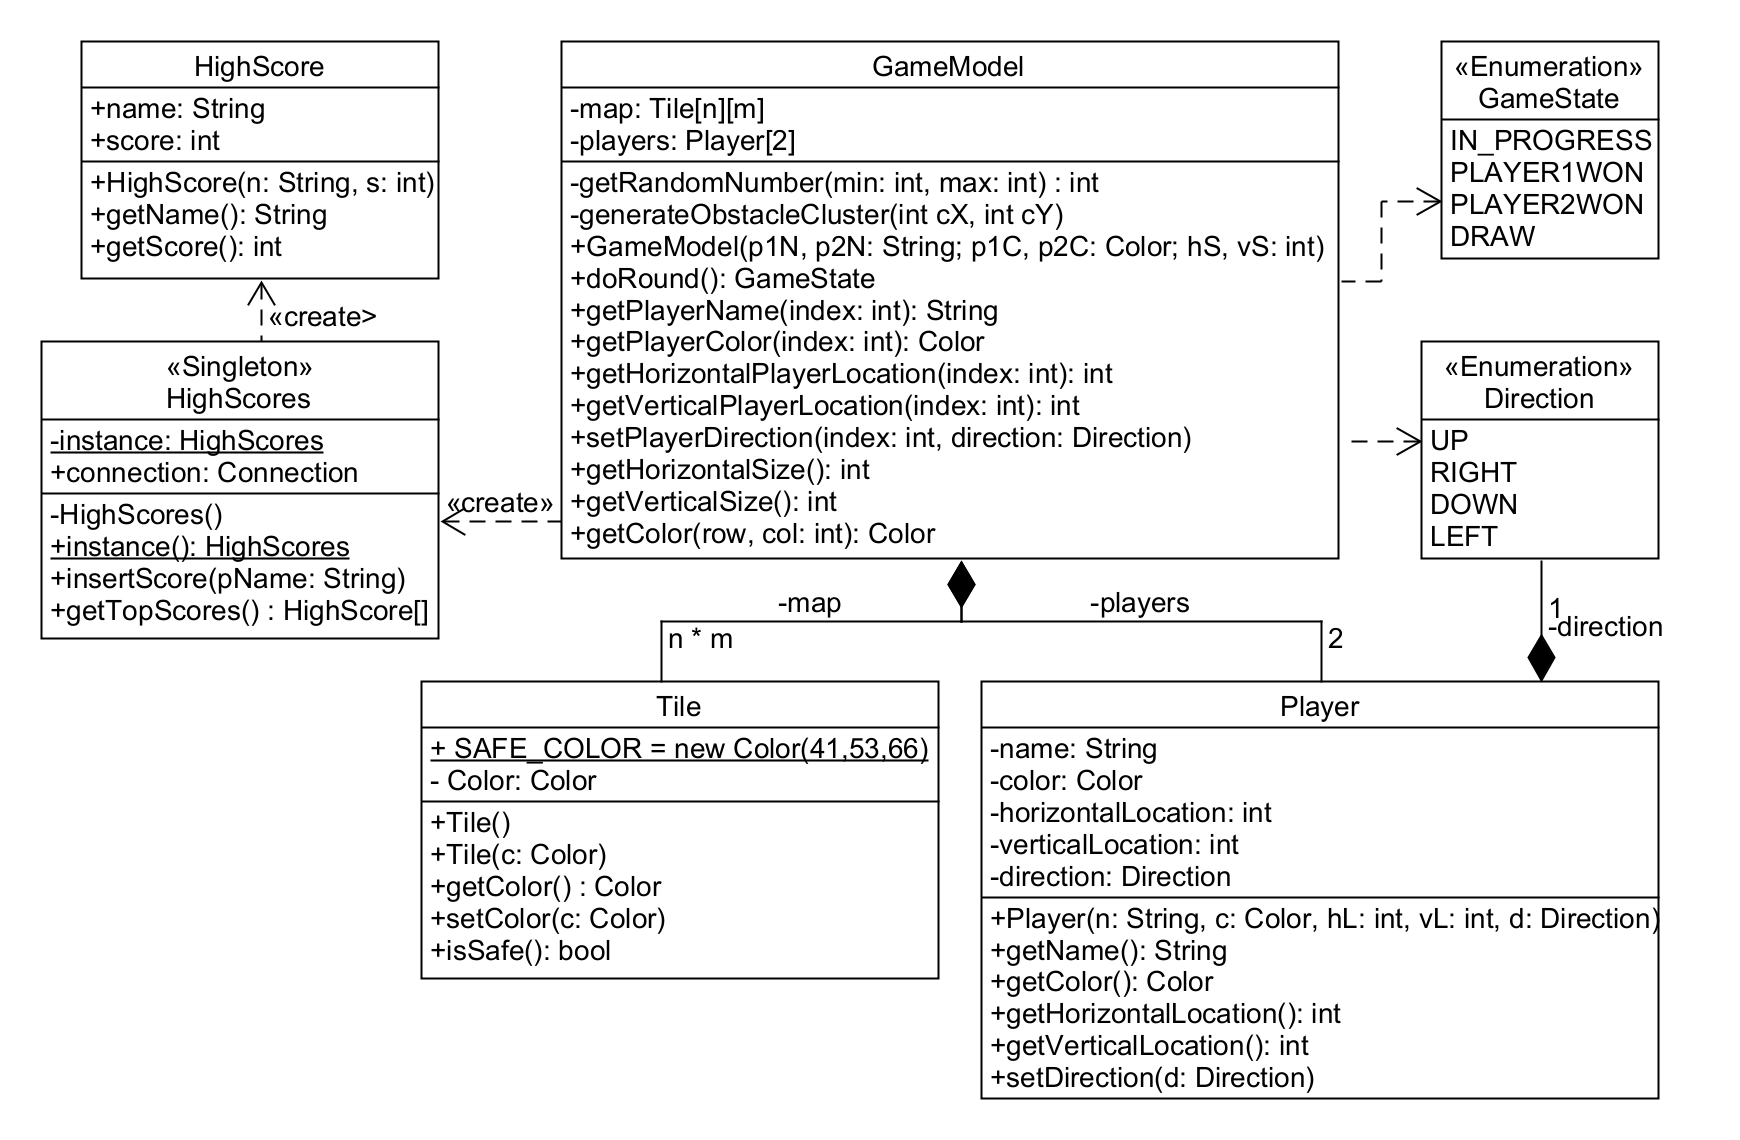
\includegraphics[scale=0.25]{model}
	\end{figure}
	\subsubsection{Nézet}
	\begin{figure}[H]
		\centering
		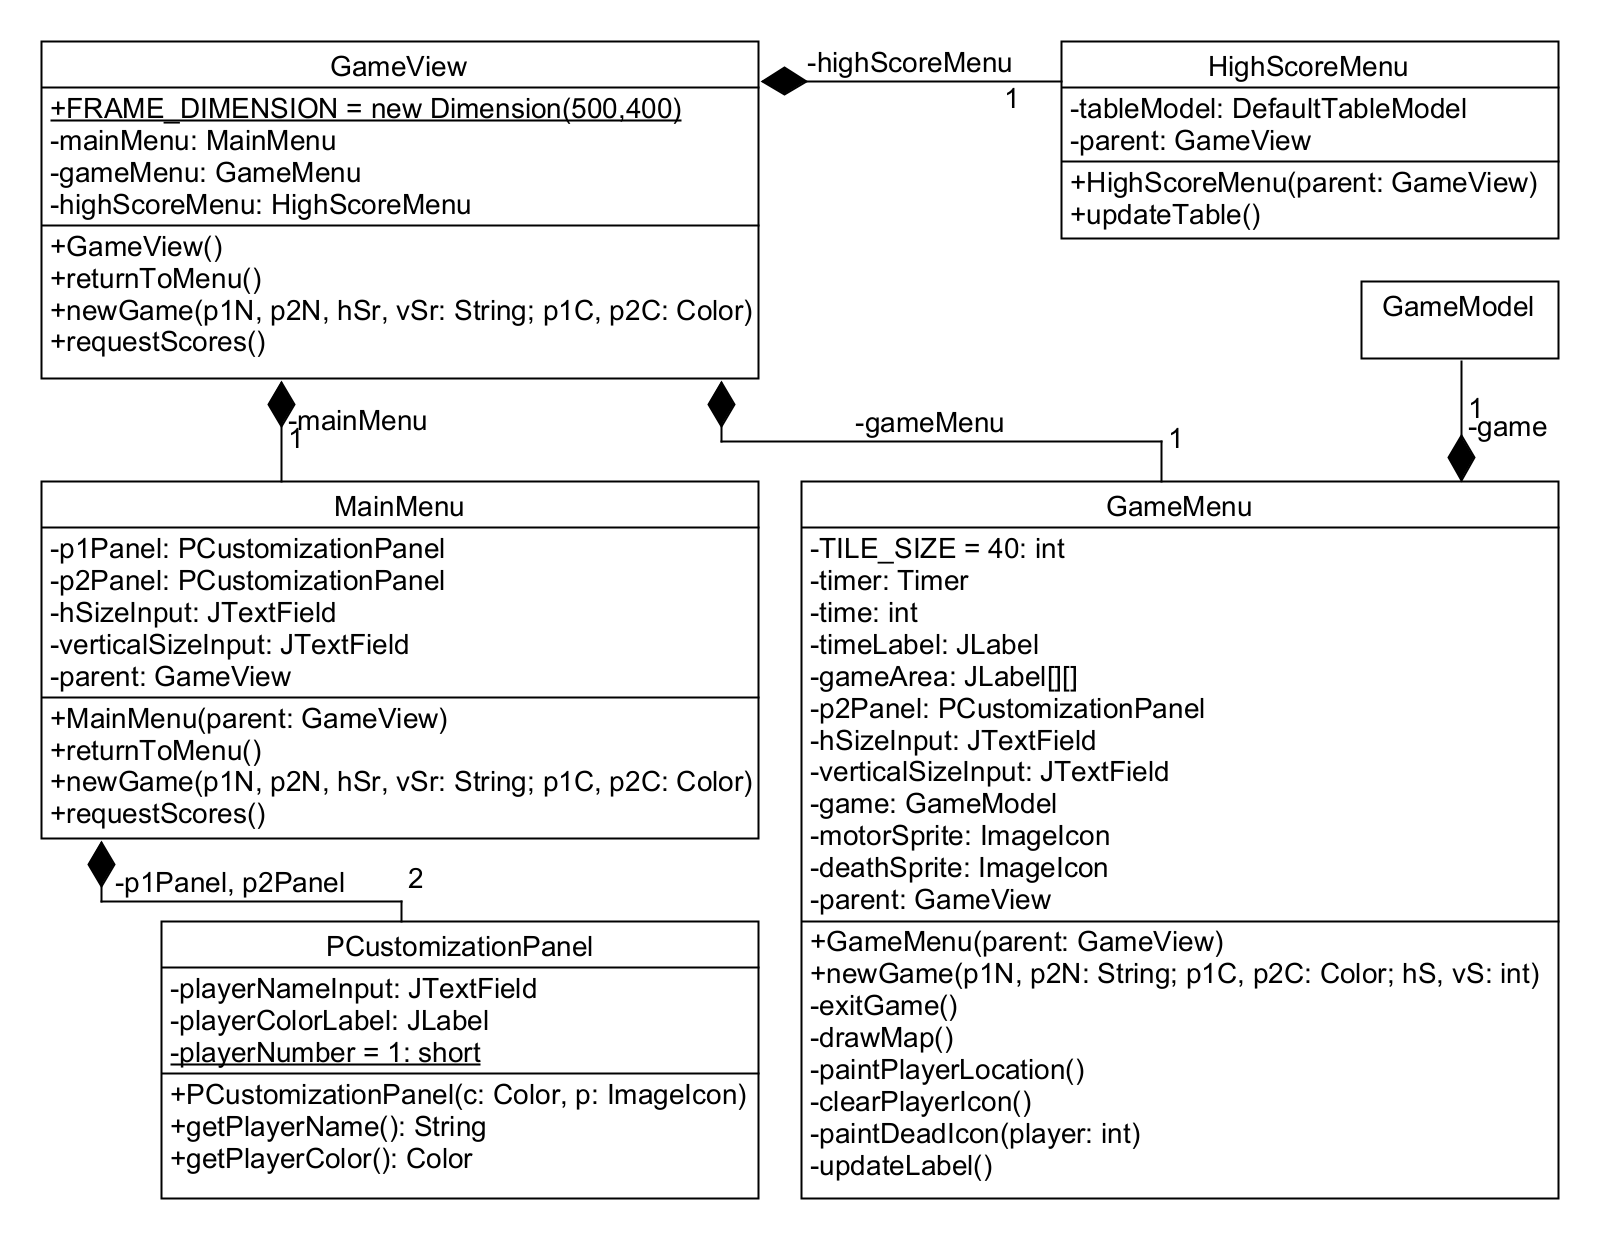
\includegraphics[scale=0.25]{view}
	\end{figure}
	\section{Tesztelés}
	\subsection{Fehérdobozos tesztesetek}
	\begin{figure}[H]	
		\centering
		\begin{tblr}{colspec={|X|X[2]|}, row{1} = {c}, hlines, cells={m,c},}
			Tevékenység            & elvárt eredmény \\
			adatbázis kapcsolat nem tud létrejönni & \mintinline{java}|SQLException| \\
			játékosnevek megegyeznek & \mintinline{java}|IllegalArgumentException| \\
			egyik játékosnév üres & \mintinline{java}|IllegalArgumentException| \\
			játékosok színe megegyezik & \mintinline{java}|IllegalArgumentException| \\
			egyik játékosok a játék számára fenntartott színt választ & \mintinline{java}|IllegalArgumentException| \\
			pályaméret túl kicsi & \mintinline{java}|IllegalArgumentException| \\
			pályaméret egyik oldala páros & \mintinline{java}|IllegalArgumentException| \\
			játékparaméterek megfelelőek & létrejön a \mintinline{java}|GameModel| objektum \\
			játék véget ér & adatbázis frissül
		\end{tblr}
	\end{figure}
	\subsection{Feketedobozos tesztesetek}
	\begin{figure}[H]	
	\centering
	\begin{tblr}{colspec={|X|X[2]|}, row{1} = {c}, hlines, cells={m,c},}
		Tevékenység            & elvárt eredmény \\
		Játékosnevek szerkesztése & új játék indításakor az új név jelenik meg \\
		Játékosszín szerkesztése & új játék indításakor az új szín jelenik meg \\
		pályaméret megadása & új játék a megadott méretek alapján jön létre \\
		hiba történik & hibaüzenet jelenik meg felugró ablakként \\
		új játék gomb megnyomása & új játék indul a megadott adatokkal \\
		eredmények gomb megnyomása & megjelennek az eredmények \\
		kilépés gomb megnyomása & a program bezáródik \\
		a játék indítása & számláló elindul, másodpercenként előrelép a játék \\
		egyik játékos ütközik & a számláló megáll, a játék véget ér, megjelenik a győztes, visszalép a főmenübe \\
		escape megnyomása játék közbe & játék félbeszakad, visszalép a főmenübe \\
		irányítóbillentyűk megnyomása játék közbe & a megfelelő játékos irányt vált \\
		vissza gomb megnyomás az eredmények menüben & visszalép a főmenübe
	\end{tblr}
\end{figure}
\end{document}